\chapter{Asynchronous Programming}

\section{Introduction: The Waiting Problem}

When developing system-level applications, we frequently encounter situations where our program must perform multiple operations concurrently. A common instinct is to reach for threads. However, before deciding on a concurrency model, we must fundamentally categorize the nature of the work our program is doing: is it \textbf{CPU-bound} or \textbf{I/O-bound}?

A \textbf{CPU-bound} task is one where the bottleneck is the processor. Examples include training AI models, performing complex matrix multiplications, or encrypting large streams of data. In these scenarios, computation can be cleanly divided into smaller chunks, and assigning each chunk to a dedicated OS thread allows us to leverage multi-core processors. The goal here is \textit{parallelism}: decreasing total execution time by doing mathematical work simultaneously across multiple cores. 

\begin{insightbox}
\textbf{The Professor's Matrix Analogy} \\
Imagine an AI system multiplying two massive matrices (e.g., 10 million rows by 10 million columns). We cannot compute this sequentially. Instead, we assign the multiplication of specific rows and columns to different threads. If we use 10 threads across multiple cores, each thread handles a chunk of the problem. Because the math is purely CPU-bound, the total execution time is drastically reduced (roughly approaching $1/N$).
\end{insightbox}

Conversely, an \textbf{I/O-bound} task spends the vast majority of its time waiting for an external subsystem to complete an operation. Imagine a program performing a deep file system search (like Windows Explorer searching the entire disk). The program must read chunks of bytes and compare strings. However, the time spent comparing strings is a marginal fraction of the time spent waiting for the disk to retrieve blocks and cross the OS barrier. If measured finely, the thread spends 99.9\% of its time parked, doing nothing.

\begin{insightbox}
\textbf{The Threading Paradox in the Cloud} \\
If we use a dedicated OS thread for every I/O-bound task, we encounter a severe inefficiency. Consider a web server like Amazon. It receives an HTTP request, decodes it, and queries a 60-year-old database. While waiting for the database, the thread sits idle. However, each thread carries a fixed cost. If you deploy your own server to the cloud, you pay for memory. If your server receives 10,000 concurrent requests and creates 10,000 threads, it consumes 10-20 Gigabytes of RAM (due to the 1-2MB stack per thread) just to \textit{wait}. We are paying for resources that are effectively doing nothing 99.9\% of the time. 

Benchmark data (e.g., Jim Blandy's experiments) highlights this disparity:
\begin{itemize}
    \item \textbf{Creation Time:} $\sim$0.3 \textmu s for an async task vs $\sim$17 \textmu s for a thread (50x slower).
    \item \textbf{Context Switch:} $\sim$0.2 \textmu s for a task vs $\sim$1.7 \textmu s for a thread (8.5x slower, due to system calls).
    \item \textbf{Memory:} 300-500 bytes for a task vs $\sim$9.5 KB of kernel data + 1-8MB stack for a thread.
\end{itemize}
\end{insightbox}

For I/O-bound tasks, we do not need more calculation speed; we need the capacity to efficiently manage thousands of concurrent \textit{waiting periods}. This is where \textbf{asynchronous programming} shines. We use threads to compute in parallel, but we use asynchronous execution to \textit{wait} in parallel.

\section{Strategies for Handling Concurrency}

To intuitively understand the difference between parallelism and concurrency, consider an analogy from a cafeteria: multi-threading is like having multiple cooks in the kitchen simultaneously preparing meals (parallel execution of CPU-bound tasks). Asynchronous concurrency is like the staff serving pasta. You do not need a dedicated server for each student in the line. A single server can rapidly hand out portions, interleaving their actions. While one student grabs their plate, the server is already serving the next. This overlap of waiting times is the essence of concurrent coordination.

Let us evaluate the three primary strategies for handling multiple I/O-bound operations (e.g., reading three files, or serving three HTTP requests):

\begin{enumerate}
    \item \textbf{Sequential Execution:} We perform Activity 1, wait for it to finish, then Activity 2, and so on. The total time is the sum of all individual times. It is easy to implement but provides unacceptable performance for the user.
    \item \textbf{Multi-threading (Preemptive):} We spawn a thread for each activity. The OS preemptive scheduler manages them. The code remains simple, but as discussed, the memory and context-switching overhead scale terribly with the number of tasks.
    \item \textbf{Asynchronous (Cooperative):} A single thread initiates Activity 1, tells the OS "let me know when the data is ready," and immediately moves on to initiate Activity 2. The thread coordinates thousands of tasks by cooperative switching: when a task cannot proceed without waiting, it explicitly yields control back to the application, allowing the thread to work on something else.
\end{enumerate}

The asynchronous approach is essentially a cooperative, application-level scheduling system. But how do we express this in code?

\section{From Callbacks to State Machines}

Historically, asynchronous behavior was implemented using \textbf{callbacks} or continuations (similar to \texttt{.then()} in JavaScript). You would instruct a system: "Start reading this file, and when you finish, execute this closure." 

While this avoids blocking the thread, callbacks suffer from severe pathologies:
\begin{itemize}
    \item \textbf{Wiring Complexity \& Error Handling:} Suppose you want to copy a file. You invoke \texttt{read\_async} and pass a continuation to invoke \texttt{write\_async}. However, \texttt{write} can fail (e.g., disk full, file deleted). The \texttt{read} might also fail before starting. What should be a trivial sequence quickly explodes into 4 or 5 complex error-handling branches. Propagating these errors across deeply nested closures is notoriously difficult.
    \item \textbf{Control Flow limits:} Implementing a simple \texttt{while} loop that performs asynchronous reads inside is nearly impossible to represent statically with simple callbacks. You cannot statically develop the combination tree for an arbitrary number of loops. The only solution is to build a complex \textbf{state machine}.
\end{itemize}

\subsection{The \texttt{async}/\texttt{await} Transformation}

Rust solves this using the \texttt{async} and \texttt{await} keywords. Instead of writing nested callbacks, we write code that looks entirely synchronous and sequential. 

\begin{lstlisting}[language=Rust]
async fn copy_file(src: &str, dst: &str) -> Result<(), std::io::Error> {
    let data = read_async(src).await?;
    write_async(dst, &data).await?;
    Ok(())
}
\end{lstlisting}

When the compiler encounters an \texttt{async fn}, it does something magical: it does not execute the function block sequentially. Instead, it transforms the entire function body into a \textbf{State Machine}. 

Every \texttt{.await} point represents a state transition---a point where the function can be paused and later resumed. The compiler achieves this by synthesizing a state machine structured as an \texttt{enum}, where each variant stores the local variables needed for that specific state:

\begin{lstlisting}[language=Rust]
enum CopySM {
    State0 { src: String, dst: String },
    State1 { dst: String, data: Vec<u8>, read_future: ... },
    State2 { write_future: ... },
    Done
}
\end{lstlisting}

1. \textbf{State 0:} Start executing until \texttt{read\_async(src).await}. The state machine saves \texttt{dst} and transitions to State 1. If the read is not ready, it yields control.
2. \textbf{State 1:} Resume once the read completes, extracting the \texttt{data}. Proceed until \texttt{write\_async(dst, \&data).await}, saving necessary futures and transitioning to State 2.
3. \textbf{State 2:} Resume once the write completes, transitioning to \texttt{Done} and returning the final result.

\begin{notebox}
\textbf{Zero-Cost Abstractions} \\
The compiler generates this state machine for you. It handles all the complex routing, variable saving (across await points), and looping. You get the readability of synchronous code with the performance of asynchronous execution.
\end{notebox}

\section{Formalizing the Mechanism: The \texttt{Future} Trait}

Because \texttt{async} functions are compiled into state machines, they do not immediately return their final value. Instead, calling an \texttt{async fn} returns an anonymous object that implements the \texttt{Future} trait.

\begin{examprioritybox}
\textbf{Futures are Inert (Lazy Evaluation)} \\
\textbf{Common Pitfall:} Calling an \texttt{async fn} and discarding the returned \texttt{Future} without \texttt{.await}ing it.\\
\textbf{Expected Mastery Level:} High. \\
The professor explicitly contrasts Rust with JavaScript. In JS, calling an async function (like \texttt{fetch}) immediately places the continuation onto the browser's single global \textbf{Message Queue}. The runtime automatically executes it. In Rust, an \texttt{async} function simply returns a state machine object (a Future). It does \textit{absolutely nothing} until it is actively polled by the executor (typically initiated by \texttt{.await}). If you forget the \texttt{.await}, the operation is silently never executed.
\end{examprioritybox}

Let's examine the core of asynchronous Rust: the \texttt{Future} trait.

\begin{lstlisting}[language=Rust]
use std::task::{Context, Poll};
use std::pin::Pin;

pub trait Future {
    type Output;
    
    fn poll(self: Pin<&mut Self>, cx: &mut Context<'_>) -> Poll<Self::Output>;
}
\end{lstlisting}

The most critical part of a Future is its \texttt{poll} method. When a Future is polled, it attempts to make progress on its internal state machine. It returns an enum:
\begin{itemize}
    \item \texttt{Poll::Ready(Output)}: The asynchronous operation has fully completed, and the final value is returned.
    \item \texttt{Poll::Pending}: The operation cannot proceed right now (e.g., still waiting for network data). The Future yields control back to the caller.
\end{itemize}

\subsection{Understanding \texttt{Pin} and \texttt{Context}}

You will notice two unusual types in the \texttt{poll} signature: \texttt{Pin} and \texttt{Context}.

\begin{itemize}
    \item \textbf{\texttt{Pin<\&mut Self>}:} Because the compiler transforms our \texttt{async} block into a state machine, local variables that are held across \texttt{.await} points must be stored inside this generated struct. Sometimes, these variables might contain references to other variables within the \textit{same} struct (self-referential structs). If the Future were moved in memory, these pointers would instantly become invalid. \texttt{Pin} is a wrapper that guarantees the object will never be moved in memory, ensuring memory safety for the state machine.
    \item \textbf{\texttt{Context<'\_>}:} When a Future returns \texttt{Poll::Pending}, how does the system know when to try polling it again? It would be terribly inefficient to constantly poll a waiting Future in a busy loop. The \texttt{Context} provides access to a \texttt{Waker}. The Future registers this \texttt{Waker} with the operating system's event listener. When the OS event occurs (e.g., data arrives on a socket), the \texttt{Waker} is triggered, signaling that this specific Future is ready to be polled again.
\end{itemize}

\subsection{Ownership Across Time}

In synchronous code, ownership is tied to the current call stack. In asynchronous code, however, a computation can suspend at an \texttt{.await} point and resume much later. Local variables that are used after the \texttt{.await} become part of the Future's internal state (as seen in our \texttt{enum} example).

If the chosen Executor is multi-threaded (like Tokio's default worker pool), it might employ \textit{work stealing}. A Future could suspend on Thread A, but later be woken up and resumed by Thread B. Consequently, ownership in async Rust crosses not just space (threads), but time. This imposes the constraint that any data held across an \texttt{.await} point must implement the \texttt{Send} trait to migrate between threads safely.

\section{Executors and the Runtime}

Rust provides the language syntax (\texttt{async}/\texttt{await}) and the standard interface (\texttt{Future} trait). However, \textbf{Rust does not provide an async runtime or a built-in message queue}. 

If a Future only advances when \texttt{poll} is called, who calls \texttt{poll}? 
This is the job of the \textbf{Executor}. 

The Executor is an application-level, cooperative scheduler. It maintains a queue of all active Futures (often called \textit{tasks}). It picks a task and calls \texttt{poll}. If it returns \texttt{Pending}, the Executor parks the task and moves on to the next one.

\begin{insightbox}
\textbf{Runtimes in the Ecosystem} \\
Because Rust leaves the runtime choice to the programmer, different domains have different standard runtimes:
\begin{itemize}
    \item \textbf{Tokio:} The heavy-duty standard for server applications. It utilizes multiple worker threads, each with its own task queue. If a worker finishes its queue, it utilizes \textit{work stealing} to take tasks from a neighbor's queue.
    \item \textbf{smol:} An extremely compact, single-threaded runtime. It has a tiny memory footprint, making it ideal for Embedded Systems where resources are tightly constrained.
    \item \textbf{async-std:} An older attempt to provide 1-to-1 asynchronous counterparts to the standard library, though it is less dominant today.
\end{itemize}
\end{insightbox}

\begin{figure}[h]
    \centering
    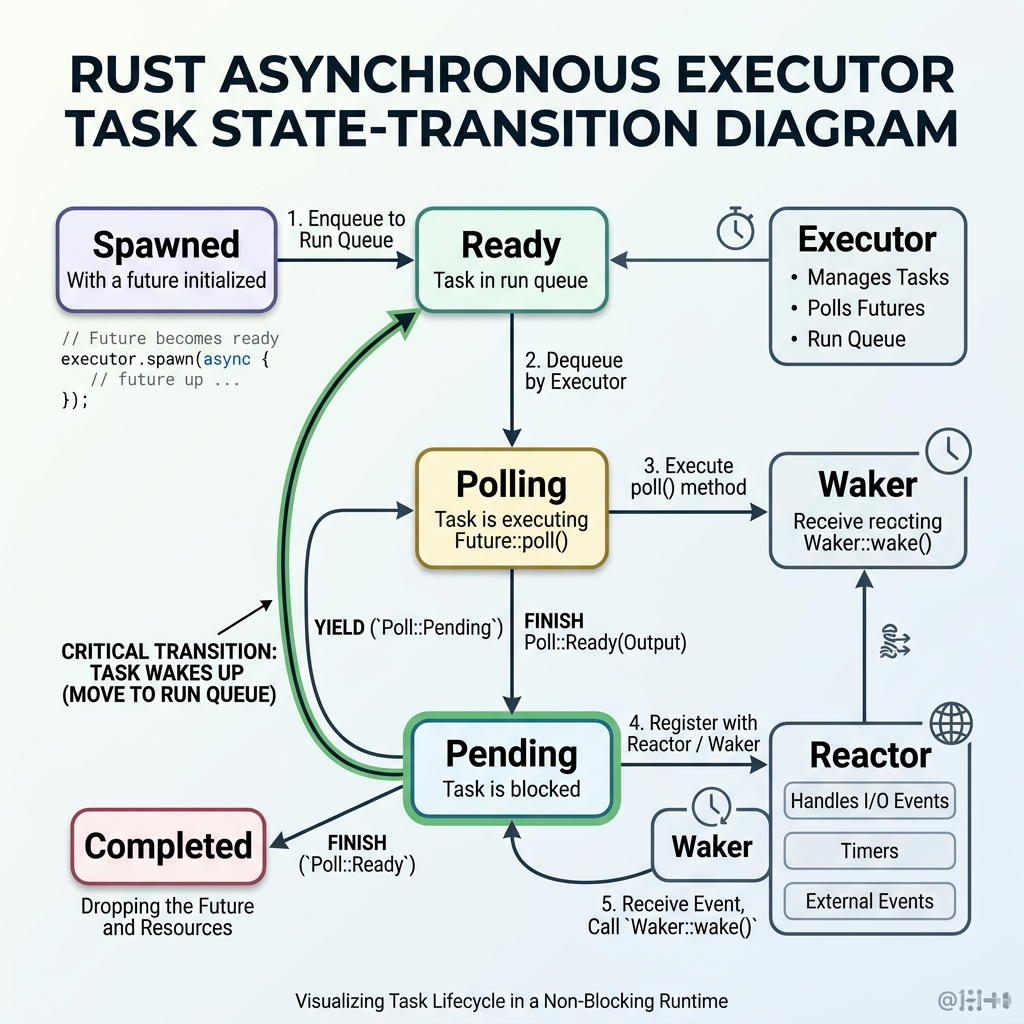
\includegraphics[width=0.8\textwidth]{images/async_executor.png}
    \caption{The Architecture of an Asynchronous Runtime}
    \label{fig:async_executor}
\end{figure}

As seen in Figure \ref{fig:async_executor}, a typical runtime consists of two parts:
\begin{enumerate}
    \item \textbf{The Executor:} Polls tasks. If a task is pending, it yields the thread back to the Executor.
    \item \textbf{The Reactor:} Interfaces with the Operating System (e.g., \texttt{epoll} on Linux, \texttt{kqueue} on macOS). When an OS I/O event completes, the Reactor uses the \texttt{Waker} to move the parked task back into the Executor's ready queue.
\end{enumerate}

\section{Working with Tokio}

Because the standard library does not include a runtime, the Rust ecosystem relies on external crates. The de-facto standard runtime is \textbf{Tokio}. It provides the Executor, the Reactor, and asynchronous versions of standard library components (like \texttt{tokio::fs} and \texttt{tokio::net}).

To start an asynchronous program, we must initialize the runtime. Tokio provides a convenient macro to transform our standard \texttt{main} function:

\begin{lstlisting}[language=Rust]
#[tokio::main]
async fn main() {
    println!("Hello from the async world!");
    
    let result = fetch_data().await;
    println!("Data: {}", result);
}

async fn fetch_data() -> String {
    // Simulating an asynchronous wait
    tokio::time::sleep(std::time::Duration::from_secs(1)).await;
    "Database payload".to_string()
}
\end{lstlisting}

Under the hood, \texttt{\#[tokio::main]} expands into a synchronous \texttt{main} function that builds the Tokio runtime and blocks the main thread while the Executor runs the \texttt{Future} generated by our \texttt{async fn main}.

\subsection{Concurrent Task Spawning}

To achieve true concurrency, we must spawn multiple independent tasks onto the Executor. This is analogous to spawning an OS thread, but we are spawning a lightweight \textit{green thread} managed by Tokio.

\begin{lstlisting}[language=Rust]
use tokio::task;

#[tokio::main]
async fn main() {
    let data = String::from("Shared payload");
    
    // Spawn a new independent asynchronous task
    let handle1 = tokio::spawn(async move {
        process_request(1, data).await;
    });

    let handle2 = tokio::spawn(async {
        process_request(2, String::from("Other")).await;
    });

    // We can await the JoinHandles to ensure they complete
    let _ = handle1.await;
    let _ = handle2.await;
}

async fn process_request(id: u32, payload: String) {
    println!("Processing request {} with payload: {}", id, payload);
    tokio::time::sleep(tokio::time::Duration::from_millis(500)).await;
    println!("Finished request {}", id);
}
\end{lstlisting}

\begin{memoryblock}
\textbf{Memory and Ownership in \texttt{tokio::spawn}}:
When you call \texttt{tokio::spawn}, Tokio dynamically allocates the task's state machine (the compiled Future) on the \textbf{heap}. This heap allocation is necessary because the task's lifetime is now decoupled from the caller's stack---the caller could return, but the background task might still be running.
Furthermore, the \texttt{async move} block forces a transfer of ownership of any captured variables (like \texttt{data}) into the Future's state machine. Because Tokio utilizes a multi-threaded work-stealing executor by default, this Future might be polled by Thread A, paused at an \texttt{.await}, and later resumed by Thread B. Consequently, every value inside the Future's state machine must implement the \texttt{Send} trait. Finally, since Tokio cannot prove how long the background task will live, any captured references would be unsafe; thus, the spawned Future is constrained by the \texttt{'static} lifetime (meaning it cannot contain borrowed references to short-lived stack variables).
\end{memoryblock}

\subsubsection{Managing Homogeneous Tasks: \texttt{JoinSet}}
If you need to spawn many tasks that all return the same type of result, managing dozens of \texttt{JoinHandle}s manually is tedious. Tokio provides the \texttt{JoinSet} structure. You can call \texttt{set.spawn()} repeatedly to add tasks to the set, and then loop over \texttt{set.join\_next().await} to process the results as they complete, in whatever order they finish.

\begin{examprioritybox}
\textbf{Blocking the Cooperative Executor} \\
\textbf{Common Pitfall:} Running heavy, synchronous CPU-bound work (like complex math, gzip compression, or blocking I/O such as \texttt{std::fs::read}) directly inside an \texttt{async} task. \\
\textbf{Expected Mastery Level:} Very High. \\
The professor repeatedly emphasizes that Tokio's scheduler is \textit{cooperative}. An \texttt{async} task must yield control by reaching an \texttt{.await} point. If a task spends hundreds of milliseconds calculating without awaiting (e.g., compressing 100,000 rows of data with gzip), it hogs the underlying worker thread. The executor cannot preempt it, meaning all other parked tasks on that thread are starved. 

For CPU-heavy work within an async application, you MUST explicitly offload it using \textbf{\texttt{tokio::task::spawn\_blocking}}. This function takes a standard closure (not an \texttt{async} block) and executes it on a dedicated, separate thread pool specifically created for blocking operations, leaving the core asynchronous worker threads free to continue polling I/O tasks.
\end{examprioritybox}

\subsection{Coordinating Tasks: \texttt{join!} and \texttt{select!}}

Often, we must coordinate multiple asynchronous tasks rather than just awaiting them in sequence. The golden rule is: \textbf{use sequential \texttt{.await}s ONLY when a task explicitly requires the result of the previous task.}

\begin{lstlisting}[language=Rust]
// Sequential execution: We MUST wait for user before fetching orders
let user = fetch_user(42).await;
let orders = fetch_orders(&user).await; 
println!("User has {} orders", orders.len());
\end{lstlisting}

If tasks are independent, awaiting them sequentially wastes time. Tokio provides powerful macros to coordinate independent tasks efficiently:

\begin{itemize}
    \item \textbf{\texttt{tokio::join!}}: Executes multiple futures concurrently on the same task. It waits for \textit{all} of them to complete and returns a tuple of their results. It is ideal when you need to fetch from multiple independent endpoints at once. Total execution time equals the longest of the tasks.
    \item \textbf{\texttt{tokio::try\_join!}}: Similar to \texttt{join!}, but if any future returns an \texttt{Err}, it aborts the others and returns the error immediately. This embraces the "all or nothing" logic.
    \item \textbf{\texttt{tokio::select!}}: Runs multiple futures simultaneously but only waits for the \textit{first} one to complete. The remaining futures are cancelled (dropped). It looks syntactically similar to a \texttt{match} statement.
\end{itemize}

\begin{usagebox}
\textbf{When and why to use coordination macros:}
\begin{itemize}
    \item \textbf{\texttt{join!} / \texttt{try\_join!}:} Use when tasks are \textit{independent} (e.g., fetching user profile and user settings) but you need \textit{all} results before proceeding. It interleaves them without spawning new worker tasks.
    \item \textbf{\texttt{select!}:} Use to handle timeouts (e.g., race a network request against a \texttt{tokio::time::sleep}) or to process whichever event arrives first on multiple channels. Canceling the slow tasks automatically cleans up resources.
\end{itemize}
\end{usagebox}

\section{Sharing State and Communicating}

When multiple spawned tasks need to interact, they face the same challenges as traditional threads. Tokio offers async-aware synchronization primitives that yield control instead of blocking the underlying OS thread.

\subsection{Shared State: \texttt{Arc<tokio::sync::Mutex<T>>}}
If tasks must mutate shared data, wrap it in Tokio's asynchronous \texttt{Mutex} paired with an \texttt{Arc}. Unlike \texttt{std::sync::Mutex}, calling \texttt{lock().await} suspends the task rather than blocking the thread, allowing the worker to execute other tasks while waiting. However, sharing memory can still create bottlenecks or lead to deadlocks.

\subsection{Message Passing: Channels}
Often, it is safer and more scalable to share data by communicating (message passing) rather than sharing memory with locks. Tokio provides several asynchronous channels:
\begin{itemize}
    \item \textbf{\texttt{oneshot} (1-to-1):} Used to send a single value. It is not repeatable. Ideal for an asynchronous task that needs to communicate a specific result to its spawner.
    \item \textbf{\texttt{mpsc} (Multi-Producer, Single-Consumer):} Used for pipelines or streaming data. Bounded \texttt{mpsc} channels provide \textit{backpressure}. For example, if a channel has a capacity of 10, the 11th \texttt{send().await} will automatically suspend the sender until the consumer processes a message.
    \item \textbf{\texttt{broadcast} (1-to-N):} One producer sends messages to many consumers. Every consumer receives a copy of \textit{all} messages.
    \item \textbf{\texttt{watch} (1-to-N):} Observes a variable and wakes up consumers when the data changes. Crucially, consumers only see the \textit{latest} value. Useful for reacting to configuration updates.
\end{itemize}

\begin{usagebox}
\textbf{When and why to use different channels:}
\begin{itemize}
    \item \textbf{\texttt{oneshot}:} When a spawned background task needs to return exactly one result to its spawner. It has zero overhead for queues.
    \item \textbf{\texttt{mpsc}:} To implement pipelines or worker queues. Crucially, bounded \texttt{mpsc} channels provide \textit{backpressure}---if the receiver is overwhelmed, senders automatically \texttt{.await} (suspend) until buffer space frees up, preventing out-of-memory crashes.
    \item \textbf{\texttt{broadcast}:} For system-wide event notifications (e.g., "Shutdown initiated") where many independent tasks need to hear the exact same message.
    \item \textbf{\texttt{watch}:} For sharing frequently updated state (like configuration settings) where receivers only care about the \textit{latest} value and can skip intermediate ones.
\end{itemize}
\end{usagebox}

\subsection*{Exam Relevance and Recurrence}
\textbf{Score: Very High.} \\
\textbf{Notes:} Asynchronous programming and Tokio are heavily tested both conceptually and practically. You must be able to explain the difference between CPU-bound and I/O-bound tasks, and why threads are inefficient for I/O. Expect questions asking you to mentally translate an \texttt{async fn} into its corresponding \texttt{enum} state machine. You will frequently be required to identify bugs where CPU-heavy code blocks the executor, or where a \texttt{Future} is dropped without being \texttt{.await}ed. 

\section{Domande ed Esercizi da Esami Passati}

\begin{exambox}
\textbf{Domanda:} Si descriva il concetto di risultato differito, come esposto dalla classe C++11 std::future<T>, indicando tre modi alternativi offerti dalla libreria standard per creare un oggetto di tale tipo e illustrando, per ciascuno di essi, un possibile caso d'uso che ne evidenzi l'utilità.
\end{exambox}

\textbf{Risposta:}
\textit{Nota: Il materiale di questo capitolo affronta il concetto di risultato differito specificamente per il linguaggio Rust, dove esso viene modellato dal trait \texttt{Future}, invece che dalla classe \texttt{std::future<T>} del C++11. Di seguito viene presentata la teoria in base ai contenuti trattati nel capitolo.}

Il concetto di risultato differito esprime un valore che non è immediatamente disponibile al momento della chiamata della funzione. Nel modello asincrono illustrato, quando si invoca una funzione \texttt{async}, essa non restituisce direttamente il risultato, ma ritorna un oggetto anonimo che implementa il trait \texttt{Future}. Questo costrutto si distingue per la sua "lazy evaluation" (valutazione pigra): il \texttt{Future} è inerte e non compie alcuna operazione se non viene attivamente interrogato (\textit{polled}) da un Executor, tipicamente attraverso l'uso della keyword \texttt{.await}. Sotto il cofano, il \texttt{Future} viene trasformato dal compilatore in una macchina a stati (spesso sotto forma di \texttt{enum}), permettendo l'esecuzione cooperativa senza bloccare il thread sottostante, una caratteristica essenziale per gestire efficientemente operazioni di I/O concorrenti.
